\section{Introduction}
\label{sec:introduction}

Composed image retrieval (CIR) turns an image and a natural-language modification into a precise visual search query. A user can provide a garment and ask for a version with a different color, texture, or silhouette. The system must preserve the relevant visual content, apply the requested change, and retrieve the intended target from a large gallery. This combination of visual retention and linguistic editing makes CIR a central test of multimodal representation learning~\cite{vo2019tirg,wufashioniq,liucirr}.

Modern CIR methods have steadily improved the query representation. Contrastive composition models align a learned multimodal query with target images~\cite{baldrati2022clip4cir}. Raw-data fusion lets a pretrained vision-language model process image-derived text and text-rendered images~\cite{wen2024dqu}. More recent systems use large multimodal models, synthetic data, explicit conflict handling, or multi-level reasoning~\cite{huynh2025collm,tian2025ccin,wang2025generative,ge2026mcot}. Their mechanisms differ, but their retrieval interface is uniform: endpoint $i$ emits a query vector $q_i$ and gallery vectors $g_i$, then ranks candidates with $q_i^\top g_i$.

This interface creates an overlooked opportunity. Consider two endpoints trained for the same CIR task. Conventional ensembling averages their matched scores, $q_0^\top g_0$ and $q_1^\top g_1$. It never evaluates $q_0^\top g_1$ or $q_1^\top g_0$. When the endpoints remain in a compatible pretrained vision-language space~\cite{radford2021clip}, these off-diagonal terms are meaningful retrieval functions. They also need not duplicate the behavior of either endpoint. A query composer can improve which semantics are retained, while a gallery encoder can improve how those semantics are indexed. Exchanging the two sides creates a path that no single endpoint exposes.

\begin{figure*}[t]
    \centering
    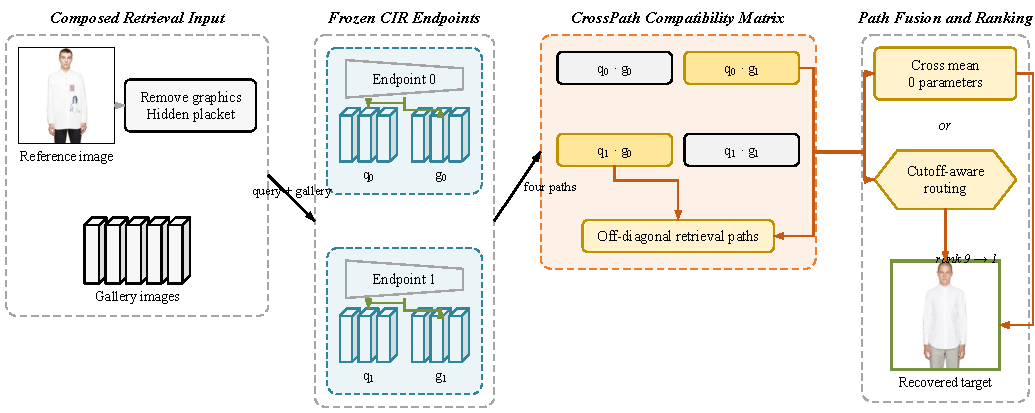
\includegraphics[width=\textwidth]{figures/fig_crosspath_framework.pdf}
    \caption{\textbf{CrossPath exposes off-diagonal compatibility between frozen CIR endpoints.} Two endpoints encode the composed query and gallery, producing four similarities $S_{ij}=q_i^\top g_j$. Standard ensembling uses only the diagonal. \method also evaluates the two cross paths and returns one ranking. In the shown FashionGen query, cross-path fusion moves the ground-truth target from rank 9 to rank 1.}
    \label{fig:framework}
\end{figure*}

We introduce \method to expose this complete compatibility space. As shown in Fig.~\ref{fig:framework}, two endpoints define a $2\times2$ score matrix. The cross mean combines its off-diagonal entries with no trainable fusion parameter. It can be applied directly when both endpoints share a coordinate-compatible embedding space, including heterogeneous CIR models built on the same pretrained representation. We also develop a routed variant for datasets whose evaluation cutoffs prefer different paths. The router operates on deterministic rank-percentile trajectories, scores only candidates whose top-$k$ membership can change, and falls back exactly to the base ranking unless the predicted utility clears a calibrated threshold.

The empirical pattern is consistent across FashionIQ~\cite{wufashioniq}, FashionGen~\cite{yuan2026fashionmv}, and the open-domain CIRR benchmark~\cite{liucirr}. On FashionIQ, combining the query side of MCoT-MVS~\cite{ge2026mcot} with DQU-CIR~\cite{wen2024dqu} gallery representations gives the strongest individual off-diagonal paths. Their cross mean improves both the strongest same-pipeline endpoint and a compute-matched diagonal ensemble. On FashionGen, the cross mean yields a large \Rone gain, while joint routing retains its early-rank strength and raises \Rfive and \Rten. CIRR contains a larger gap between the two endpoints, so a conservative one-sided cross path is more effective than an equal-weight mean. Coupling this path with query-conditioned target refinement improves the MCoT validation Avg by 0.74 points. We further apply a shared signed permutation to one endpoint's query and gallery coordinates. This operation leaves every within-endpoint dot product unchanged, but destroys cross-coordinate correspondence. Cross-path recall then falls almost to zero on FashionIQ and FashionGen. The control identifies a concrete mechanism rather than attributing the improvement to generic model averaging.

Our contributions are threefold:
\begin{itemize}
    \item We formulate endpoint composition as a complete query-gallery compatibility matrix and identify its off-diagonal paths as a source of reusable CIR ability.
    \item We present a zero-parameter cross-path reducer and a lightweight cutoff-aware router that produce one standard ranking while retaining a compute-matched diagonal ensemble as the central control.
    \item We establish gains on FashionIQ, FashionGen, and CIRR, supported by module ablations, directional path analysis, an invariance-preserving scrambling control, efficiency measurements, and retrieval visualizations.
\end{itemize}
